\chapter{Strømforsyning}
Ud fra kravspecifikation skal delmodulerne (SM og VBTE) kunne drives fra en 24V AC forsynings kilde. Selve modulerne er designet til 12V DC og 5V DC forsyningsspændringer , der designes derfor en strømforsyning der regulere spændingen så den kan levere 12V 1A og 5V 0,5A.  
\section{Krav til strømforsyning}
Indgangsspændning / Strøm: \textbf{24V AC RMS / 1,5A} \\
Udgangsspændning / Strøm: \textbf{12V DC / 1A} \\
Udgangsspændning / Strøm: \textbf{5V DC / 0,5A} \\

\section{Overordnet design}
I dette afsnit beskrives og vises det overordnede hardware blokdiagram over strømforsyningen samt beskrivelse signaler.
\begin{figure}[H]
\centering
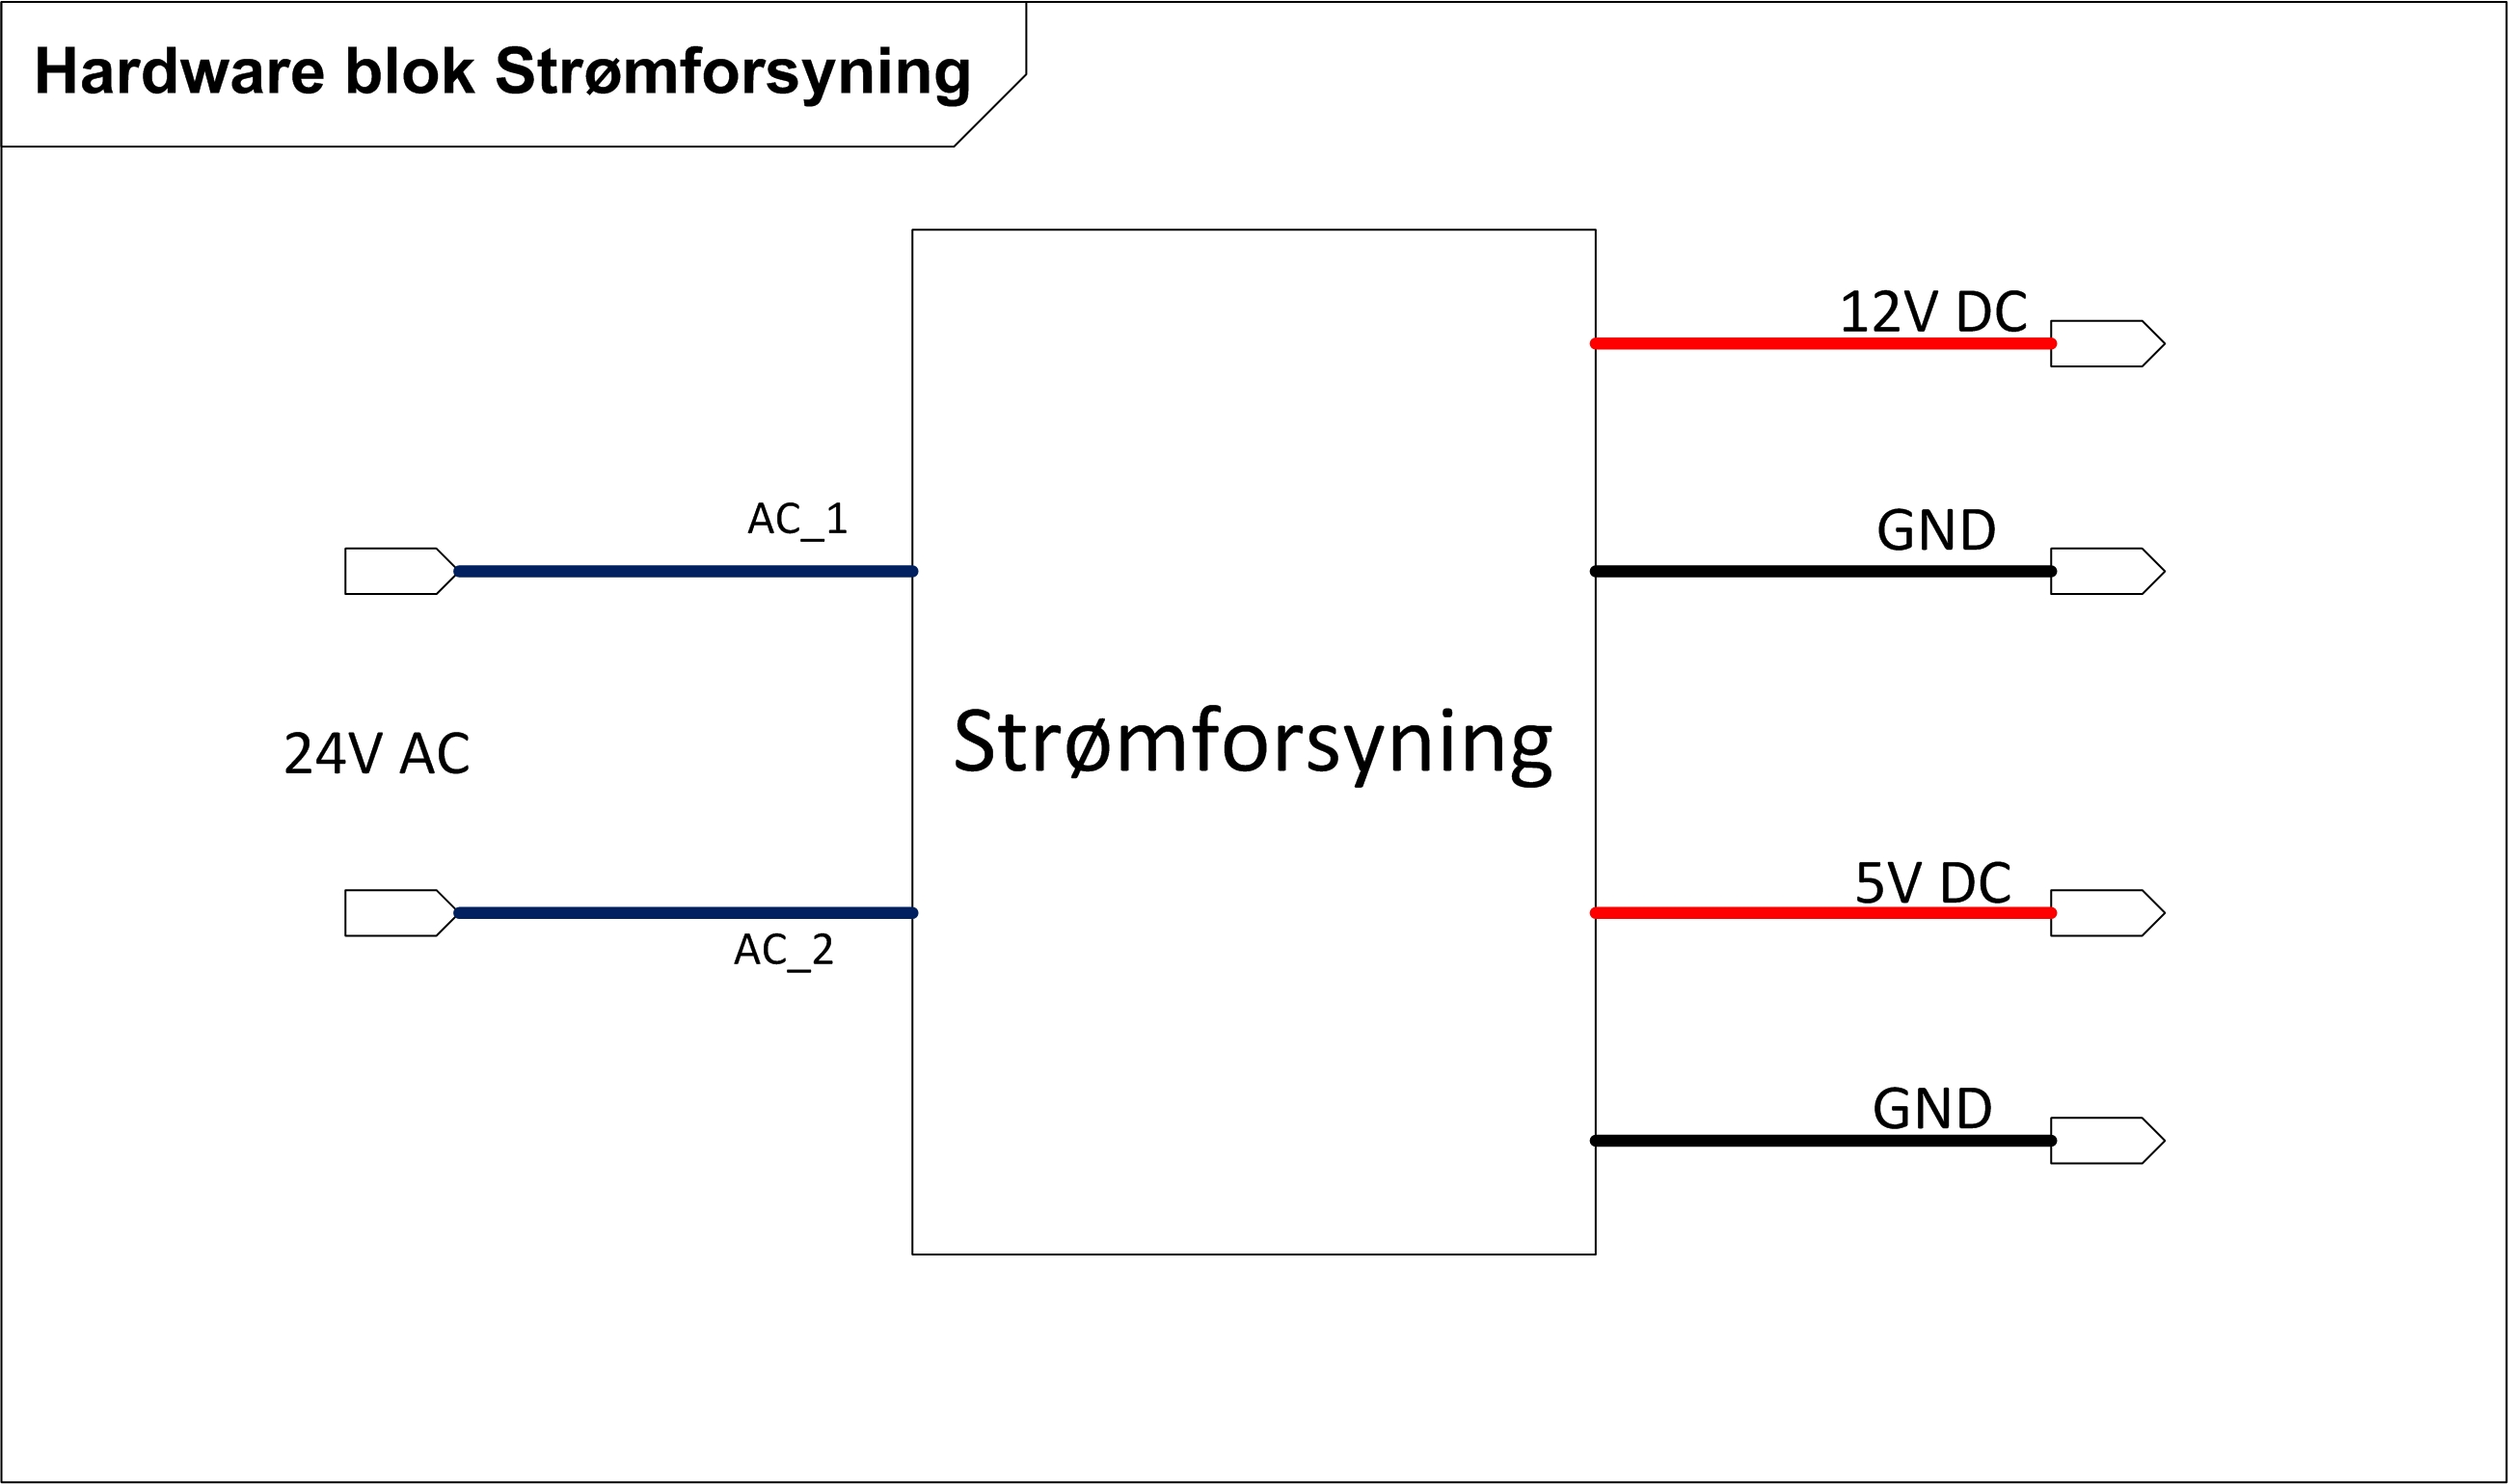
\includegraphics[scale=0.6]{billeder/PowerSupply}
\caption{Strømforsyning}
\label{fig:PowerSubbly}
\end{figure}
\begin{figure}[H]
\centering
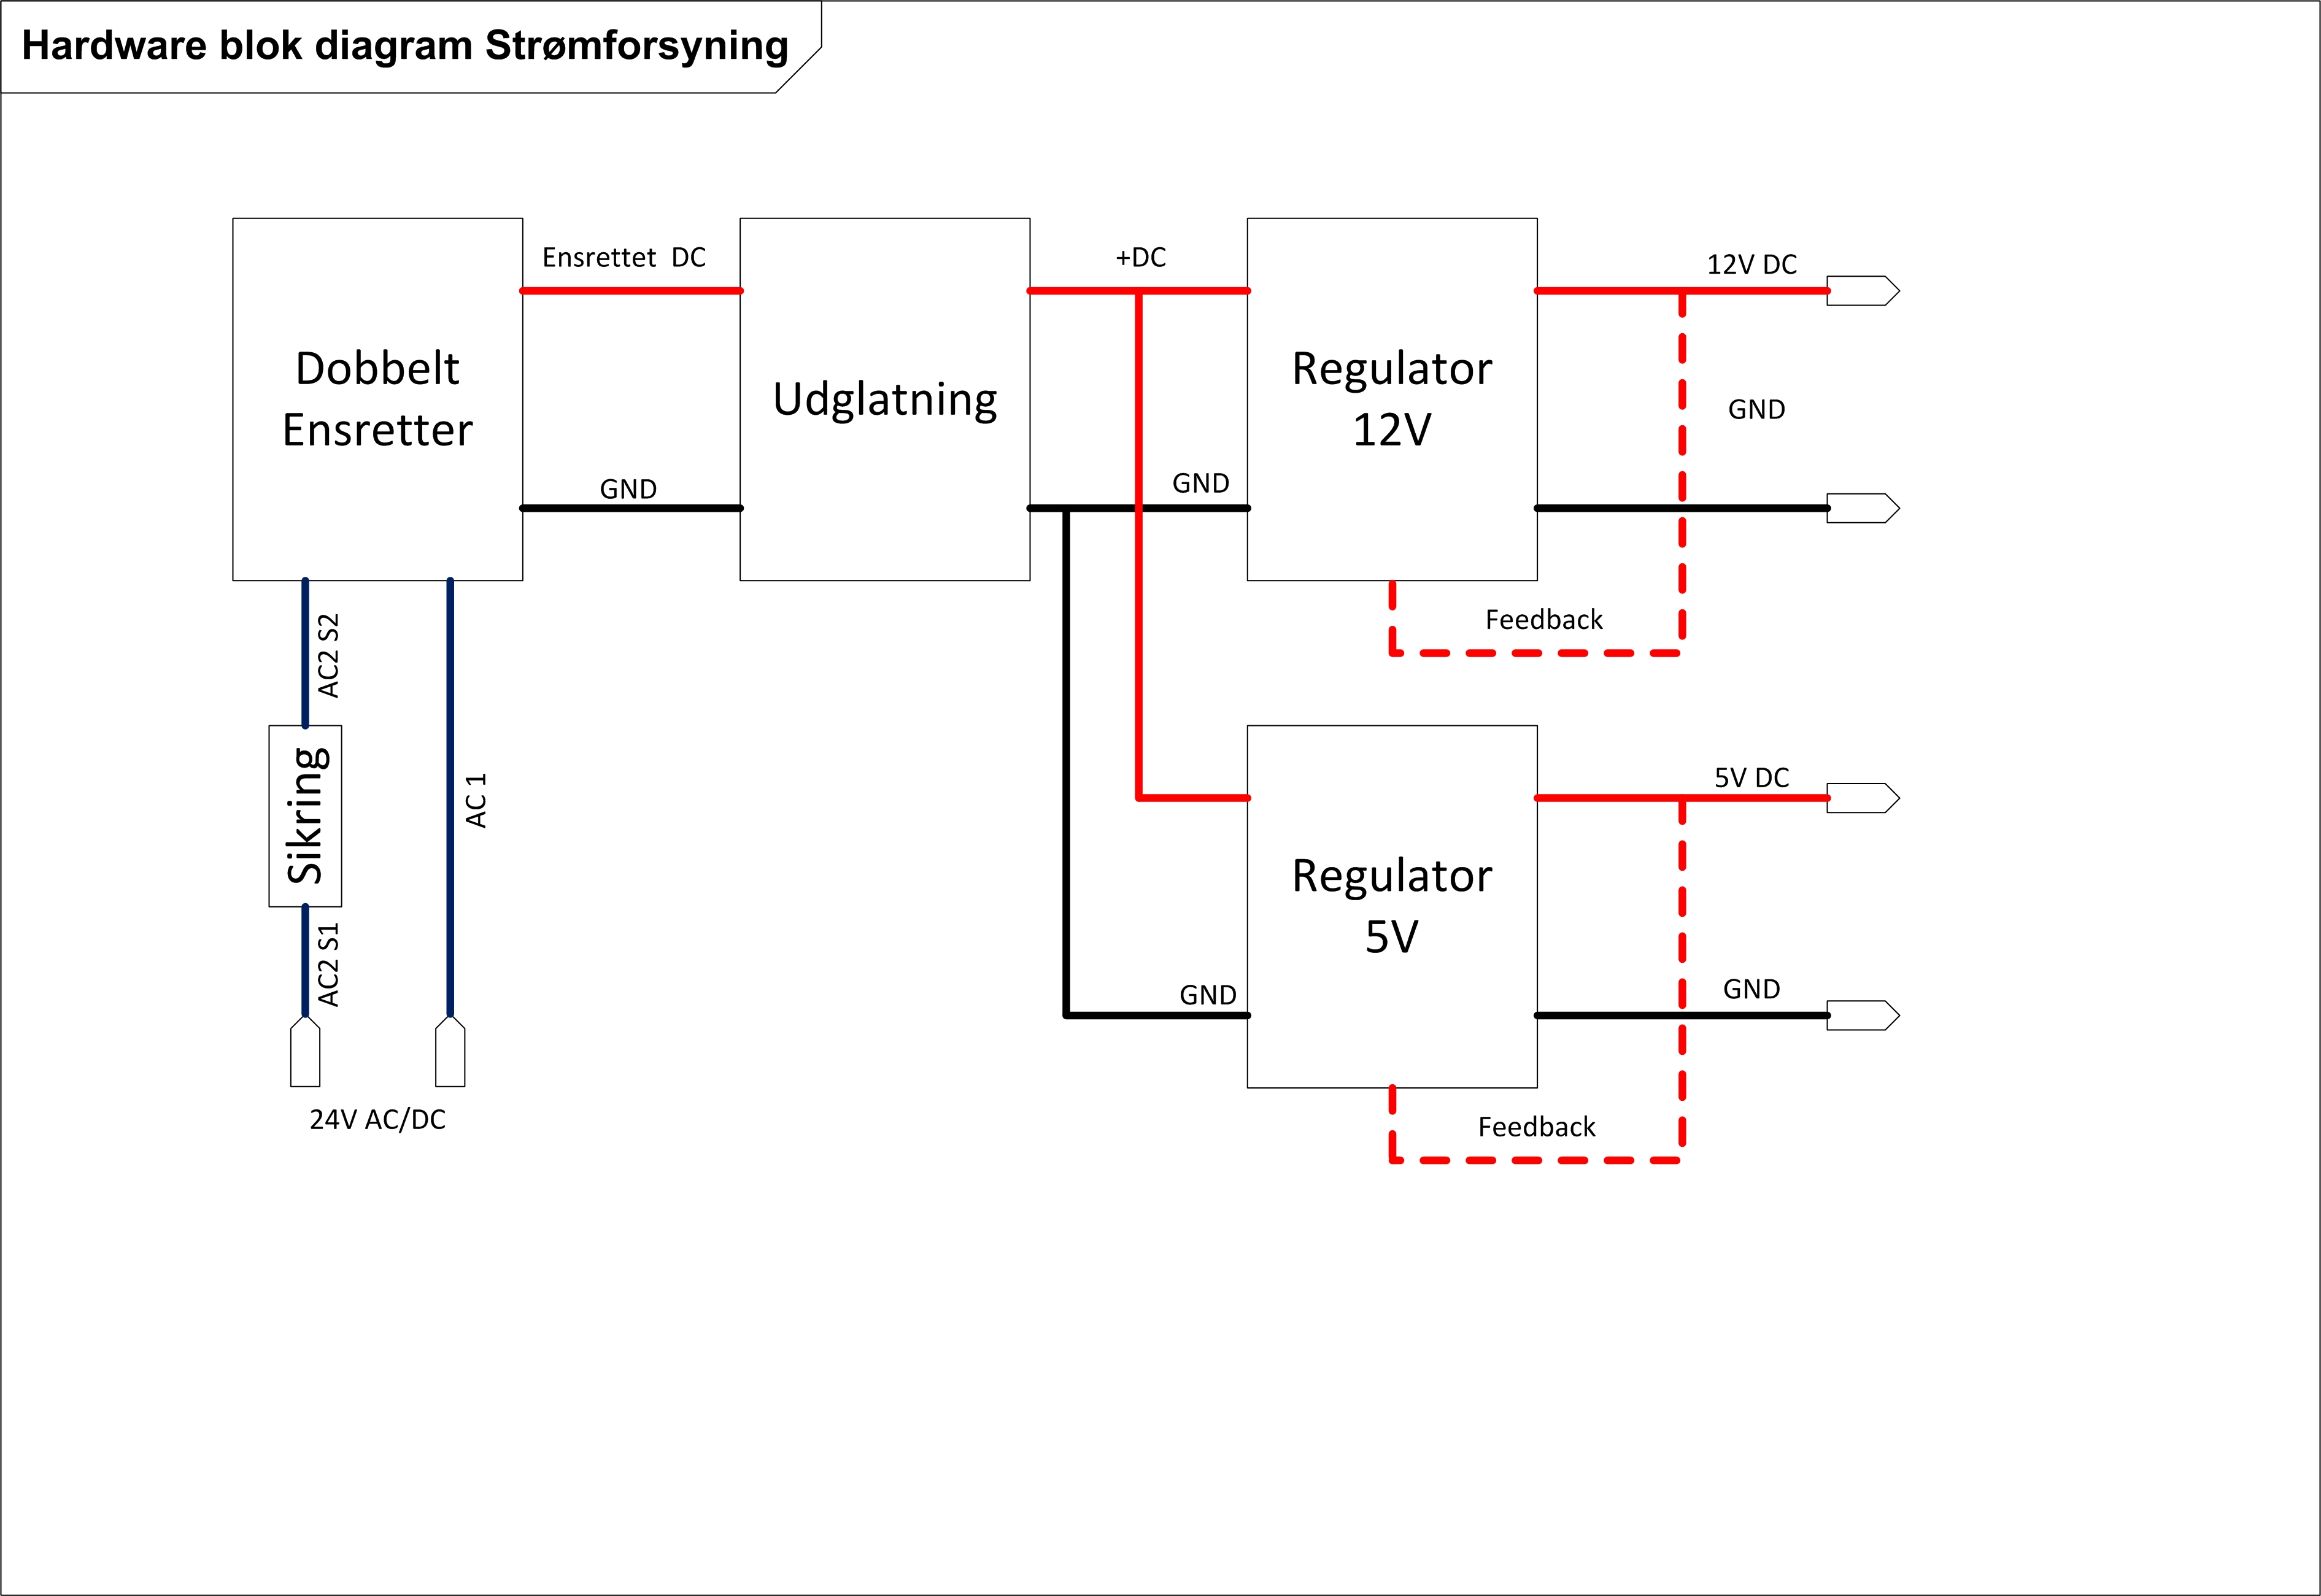
\includegraphics[scale=0.8]{billeder/PowerSupplyBlok}
\caption{Overordnet blokdiagram for strømforsyning}
\label{fig:PowerSubbly Blok}
\end{figure}
\subsection{Blokke}
Nedenfor beskrives de enkelte blokke illustreret på \textit{Figur~\ref{fig:PowerSubbly Blok}}
\subsubsection{Sikring}
Sikringen beskytter forsyningskilde, hvis der bliver for stor belastning på strømforsyningen
\subsubsection{Dobbelt ensretter}
Ensretter AC spændingen fra forsyningskilden.
\subsubsection{Udglatning}
Udglatter det ensrettet signal til en stabil positiv DC. 
\subsubsection{Regulator 12V}
Regulere den ensrettet DC ned til 12V DC.
\subsubsection{Regulator 5V}
Regulere den ensrettet DC ned til 5V DC.
\newpage
\section{Nedbrydning af blokke}
For at gøre designet af de forskellige blokke mere overskuelig nedbrydes de enkle blokke fra det overordnede blokdiagram.
\subsection{Sikring}
\begin{figure}[H]
\centering
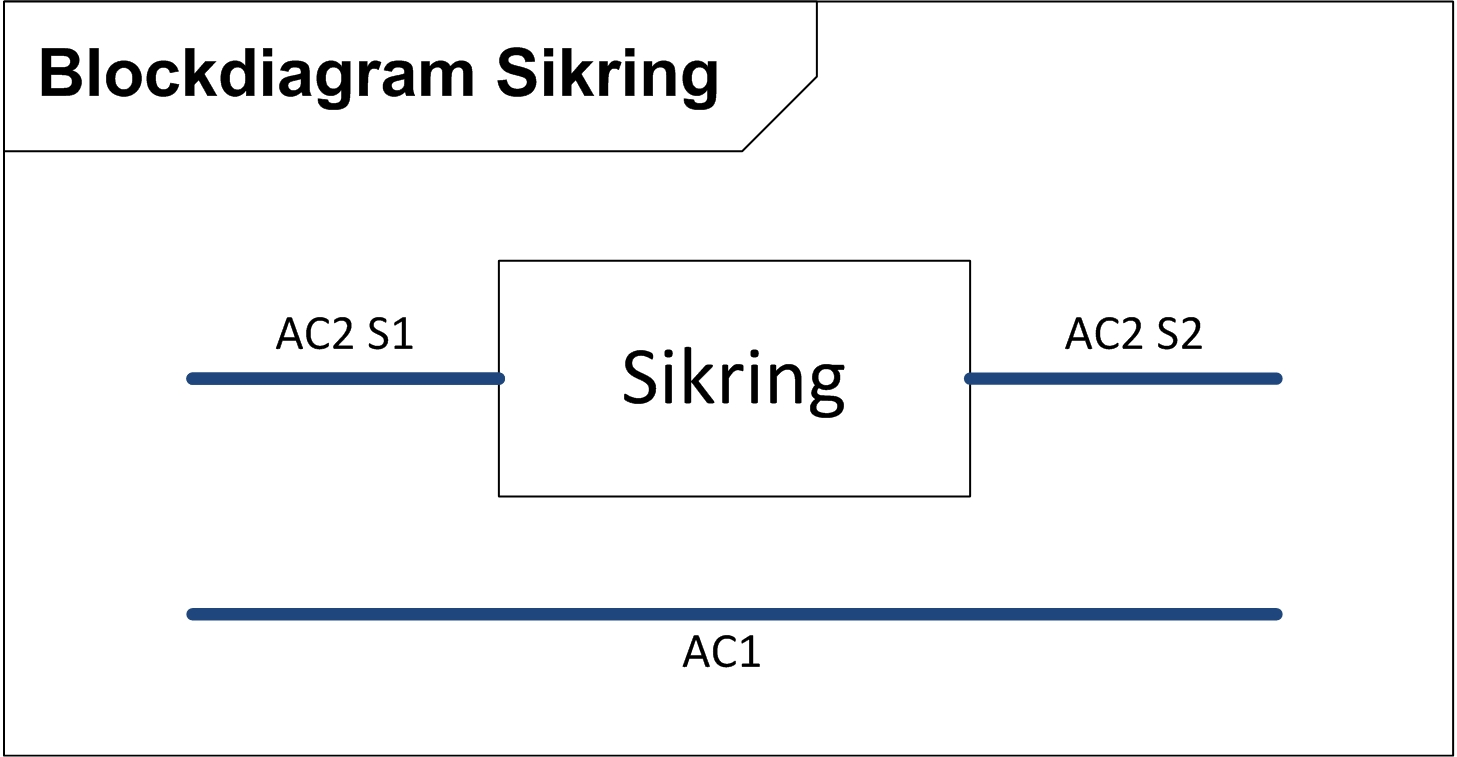
\includegraphics[scale=1]{billeder/SikringsBlok}
\caption{Blokdiagram for Sikrings blok}
\label{fig:SikringsBlok}
\end{figure}
\subsubsection{Signalbeskrivelser}
I tabellen beskrives de interne signaler
\begin{table}[H]
\begin{tabular}{|p{3cm}|p{3cm}|p{3cm}|p{4.5cm}|} \hline
\cellcolor[gray]{0.85}Signal navn& \cellcolor[gray]{0.85}Type &\cellcolor[gray]{0.85}Spænding&\cellcolor[gray]{0.85}Beskrivelse\\ \hline
AC\_1 S1 & Analog  & 24V AC RMS & Indgangsspænding fra spændingskilde inden sikring.\\  \hline
AC\_1 S2 & Analog & 24V AC RMS & Indgangsspænding fra spændingskilde efter sikring. \\  \hline
AC\_2 & Analog & 0V AC & 0V AC fra spændingskilden.\\  \hline

\end{tabular}
\caption{Tabel over signaler i Sikring}
\label{table:SikringSignaler}
\end{table}
\newpage
\subsection{Dobbelt ensretter}
\begin{figure}[H]
\centering
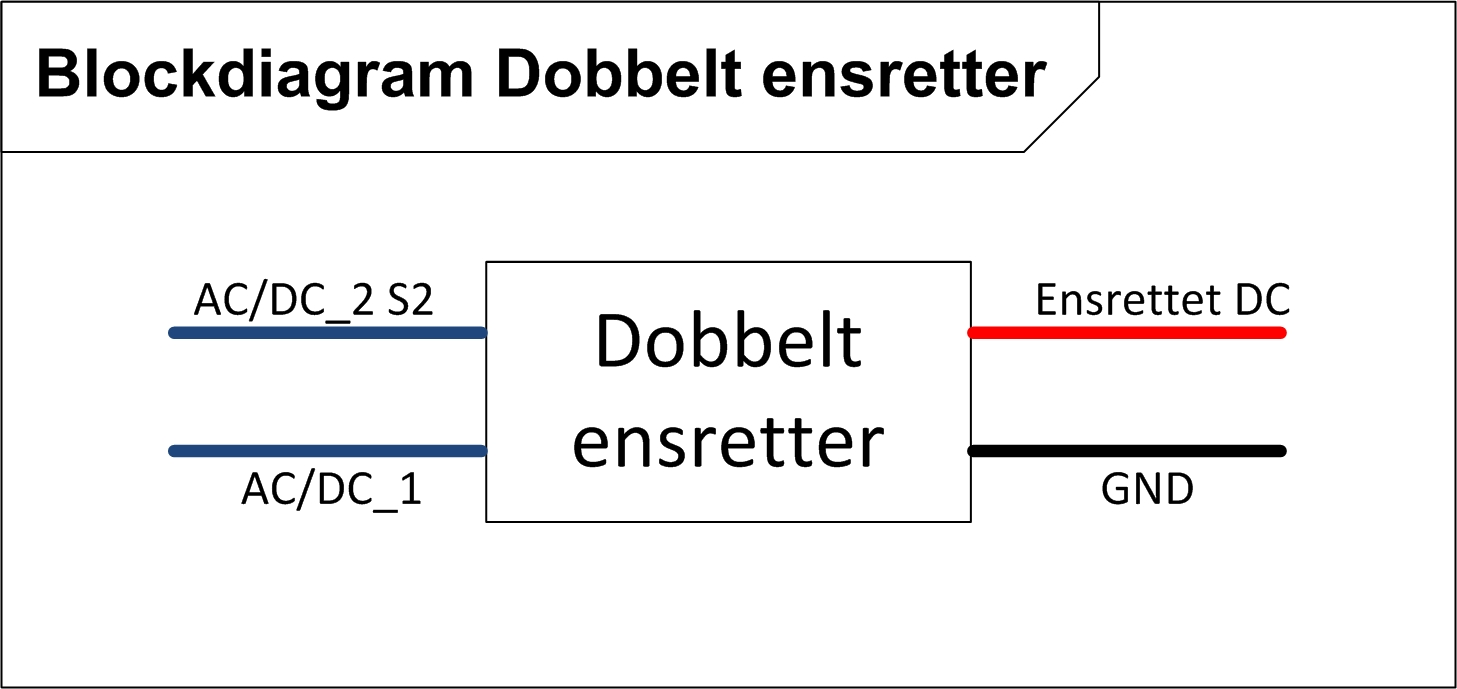
\includegraphics[scale=1]{billeder/DobbeltensretterBlok}
\caption{Blokdiagram for Dobbelt ensretter}
\label{fig:DobbeltensretterBlok}
\end{figure}
\subsubsection{Signalbeskrivelser}
I tabellen beskrives de interne signaler
\begin{table}[H]
\begin{tabular}{|p{3cm}|p{3cm}|p{3cm}|p{4.5cm}|} \hline
\cellcolor[gray]{0.85}Signal navn& \cellcolor[gray]{0.85}Type &\cellcolor[gray]{0.85}Spænding&\cellcolor[gray]{0.85}Beskrivelse\\ \hline
AC\_1 S2 & Analog  & 24V AC & Indgangsspænding fra spændingskilde efter sikring.\\  \hline
AC\_2  & Analog & 0V AC / 0V DC & 0V AC fra spændingskilden. \\  \hline
Ensrettet DC & Analog & 33 Vpk. & Det ensrettet signal består af positive halvbuer. \\ \hline
GND & Analog & 0V & Ground signal.\\ \hline
\end{tabular}
\caption{Tabel over signaler i Sikring}
\label{table:Ensretter}
\end{table}
\newpage
\subsection{Udglatning}
Udglatningen genere et jærn og stabilt DC-niveau
\begin{figure}[H]
\centering
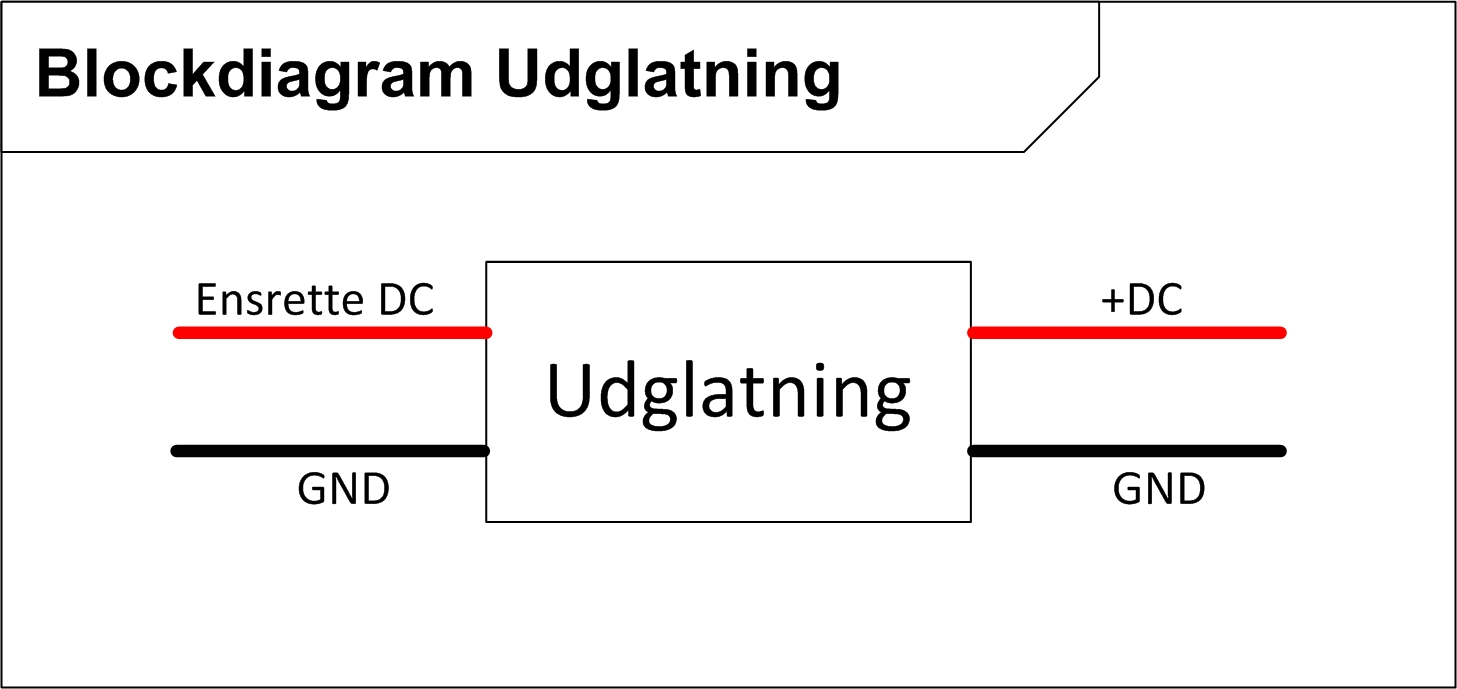
\includegraphics[scale=1]{billeder/UdglatningsBlok}
\caption{Blokdiagram for udglatning}
\label{fig:UdglatningBlok}
\end{figure}
\subsubsection{Signalbeskrivelser}
I tabellen beskrives de interne signaler.
\begin{table}[H]
\begin{tabular}{|p{3cm}|p{3cm}|p{3cm}|p{4.5cm}|} \hline
\cellcolor[gray]{0.85}Signal navn& \cellcolor[gray]{0.85}Type &\cellcolor[gray]{0.85}Spænding&\cellcolor[gray]{0.85}Beskrivelse\\ \hline
Ensrettet DC & Analog  & ca. 33 Vpk & Det ensrettet signal består af positive halvbuer. \\  \hline
GND  & Analog & 0V DC & ground signal. \\  \hline
+DC & Analog & ca. 33V DC & Jævnt og stabilt DC-niveau\\ \hline
GND & Analog & 0V DC & ground signal.\\ \hline
\end{tabular}
\caption{Tabel over signaler i Udglatning}
\label{table:udglatning}
\end{table}
\newpage
\subsection{Regulator 12V}
Regulere spædning ned til 12V DC, 1A
\begin{figure}[H]
\centering
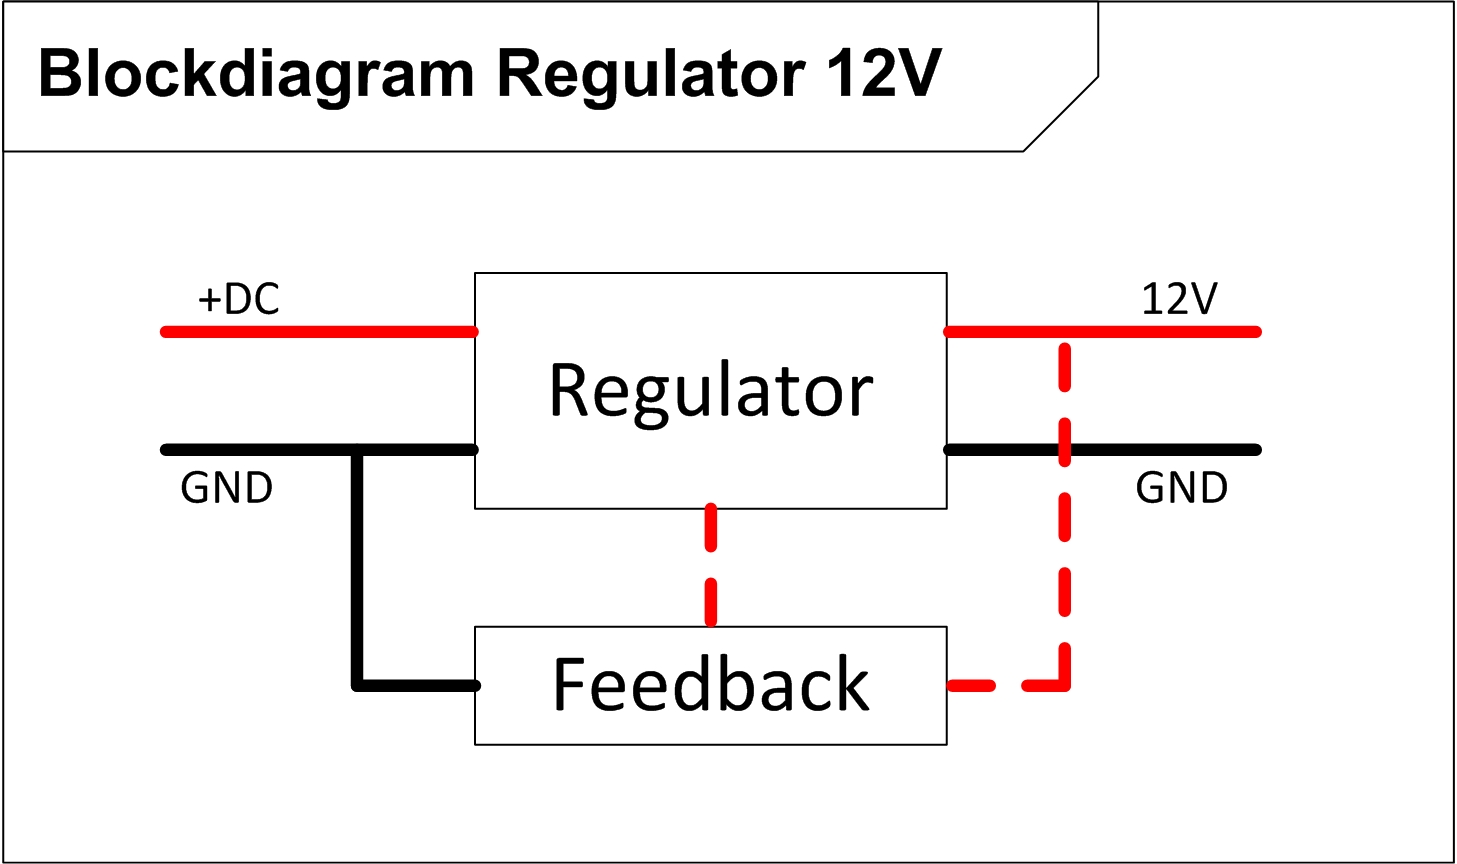
\includegraphics[scale=1]{billeder/Regulering_12VBlok}
\caption{Blokdiagram for regulator 12V}
\label{fig:regulator_12V}
\end{figure}
\subsubsection{Signalbeskrivelser}
I tabellen beskrives de interne signaler.
\begin{table}[H]
\begin{tabular}{|p{3cm}|p{3cm}|p{3cm}|p{4.5cm}|} \hline
\cellcolor[gray]{0.85}Signal navn& \cellcolor[gray]{0.85}Type &\cellcolor[gray]{0.85}Spænding&\cellcolor[gray]{0.85}Beskrivelse\\ \hline
+DC & Analog & ca. 33 VDC & jævnt og stabilt DC-niveau\\  \hline
GND  & Analog & 0V DC & ground signal. \\  \hline
12V & Analog & 12V +-0.2V & jævnt og stabilt DC-niveau\\ \hline
GND & Analog & 0V DC & ground signal.\\ \hline
Feedback\_udgang & Analog & 12V +-0.2V & Feedback signalet måler på 12V udgangen.\\ \hline
\end{tabular}
\caption{Tabel over signaler i Sikring}
\label{table:udglatning}
\end{table}
\subsubsection{Blokbeskrivelser}
\subsubsection{Regulator}
Regulatoren regulere spænding ned til 12V, de 12V er bestemt ud fra hvad feedbacket. 
\subsubsection{Feedback}
Feedbacket måler på udgangssignalet af regulatoren, feedbacket bestemmet hvilke spændning regulatoren skal indstille sig på.
\newpage
\subsection{Regulator 5V}
Regulere spædning ned til 5V DC, 0.5A
\begin{figure}[H]
\centering
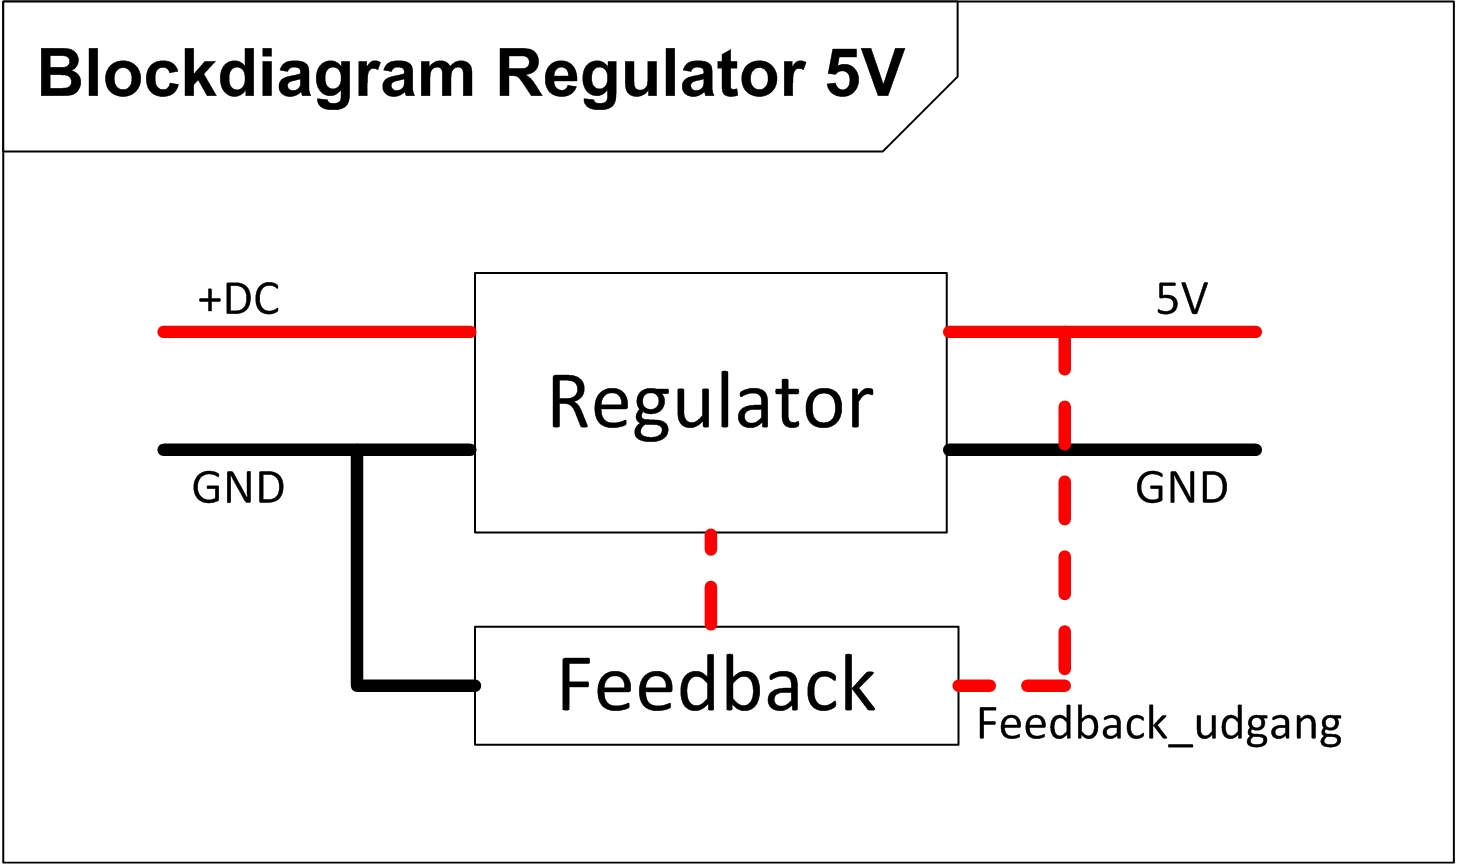
\includegraphics[scale=1]{billeder/Regulering_5VBlok}
\caption{Blokdiagram for regulator 5V}
\label{fig:regulator_5V}
\end{figure}
\subsubsection{Signalbeskrivelser}
I tabellen beskrives de interne signaler.
\begin{table}[H]
\begin{tabular}{|p{3cm}|p{3cm}|p{3cm}|p{4.5cm}|} \hline
\cellcolor[gray]{0.85}Signal navn& \cellcolor[gray]{0.85}Type &\cellcolor[gray]{0.85}Spænding&\cellcolor[gray]{0.85}Beskrivelse\\ \hline
+DC & Analog & ca. 33 VDC & jævnt og stabilt DC-niveau\\  \hline
GND  & Analog & 0V DC & ground signal. \\  \hline
12V & Analog & 5V +-0.2V & jævnt og stabilt DC-niveau\\ \hline
GND & Analog & 0V DC & ground signal.\\ \hline
Feedback\_udgang & Analog & 5V +-0.2V & Feedback signalet måler på 12V udgangen.\\ \hline
\end{tabular}
\caption{Tabel over signaler i Sikring}
\label{table:udglatning}
\end{table}
\subsubsection{Blokbeskrivelser}
\subsubsection{Regulator}
Regulatoren regulere spænding ned til 5V, de 5V er bestemt ud fra hvad feedbacket. 
\subsubsection{Feedback}
Feedbacket måler på udgangssignalet af regulatoren, feedbacket bestemmet hvilke spændning regulatoren skal indstille sig på.
\newpage
\section{Opbygning af design}
Nedenfor følger opbygningen af designet for de forskellige blokke i strømforsyningen. Dette vil blive beskrevet med Multisim designs, simuleringer, samt udregninger. 

\subsection{Sikring}
Sikringen sidder som sagt som beskyttelse af forsyningsspændningen, hvis der trækkes en for stor strøm fra strømforyningen i et kort tid vil sikringen springe. Sikringen beskytter også derfor evt. komponenter på strømforsyningen. Bestemmelsen af sikringsstørrelse sker ud fra et skema samt kortslutningsstrømmen. Kortslutningsstrømmen beregnes udfra den indre modstand i strømforsyningen og tomgangs peak spændingen: \\
\begin{figure}[H]
\centering
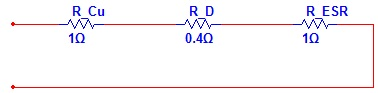
\includegraphics[scale=0.8]{billeder/Indre_modstand}
\caption{Indre modstand for Transformator, Diodebro og Elektrolyt}
\label{fig:Indre_modstand}
\end{figure}
Transformator(Forsyningskilde) R\_Cu: ca. 1 ohm \\
Dobbelt ensretter(diodebro) R\_D: 2 * 0,02 ohm = 0,04 ohm \\
Udglatning(Elektrolyt kondensator) R\_ESR: ca. 1 ohm \\
Indre modstand R\_Z = \textbf{2,04 ohm}\\ \
Peak spænding:\\
Vpk = 24V RMS*1,41 = \textbf{33,84 Vpk} \\
Kortslutningstrøm:\\
I\_K = Vpk / R\_Z = 33,84Vpk / 2,04 ohm = \textbf{16,5 A} \\
\newpage 
Ud fra beregningerne og \textit{Figur~\ref{fig:Sikringskurve_PS}} kan størrelse af sikringen findes 
\begin{figure}[H]
\centering
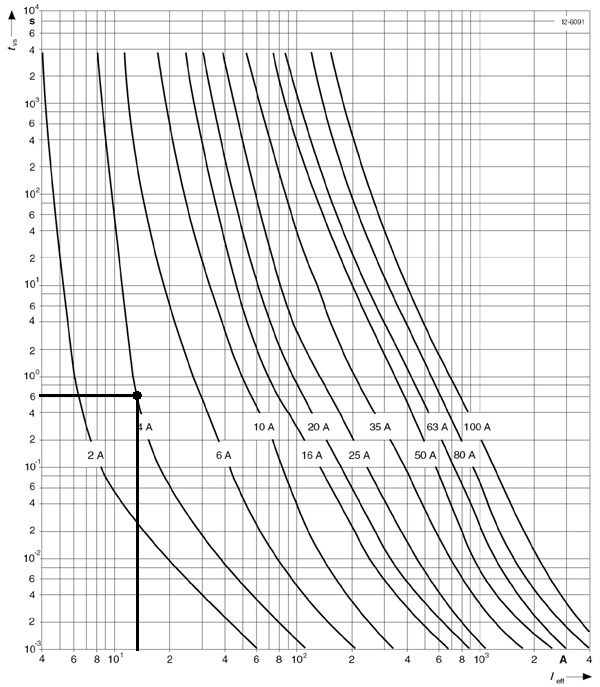
\includegraphics[scale=0.7]{billeder/Sikringskurve_PS}
\caption{Sikringskurve}
\label{fig:Sikringskurve_PS}
\end{figure}
Størrelse på sikringen vælges til \textbf{4A} og en springetid på \textbf{250ms.}
\subsection{Dobbelt ensretter}
Dobbelt ensretteren, ensretter AC signalet til positive halvperioder, ved at det er en diodebro der består af 4 dioder vil der altid være 2 dioder der leder samtidig, dette betyder at der vil være det dobbelt af positive halvperioder. Ved at der er det dobbelt af positive halvperioder betyder også en bedre udglatning af DC signalet, samt bedre udnytelse af AC signalet.
\newpage
\subsubsection{Beregning}
Spændning over diode i diodebro:\\
D\_f = 0,7V, D\_f vil stige i forhold til den strøm der løber igennem dioden\\
Peak spændning efter dobbelt ensretter:\\
Vpk\_Diodebro = (24V AC RMS * 1,41) - (2 * 0,7V) = 32,43V pk.\\
Diodenbroen der er valgt er \textbf{kbl-04} der kan klare op til 4A. 
\footnote{Se datablad for kbl-04 i bilag}
\newpage


\subsection{Udglatning}
Udglatningen består af en elektrolyt, som bliver opladet når spændning stiger og aflades når spændningen falder.
\begin{figure}[H]
\centering
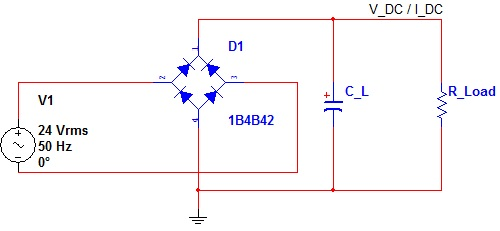
\includegraphics[scale=0.7]{billeder/Udglatning}
\caption{Diagram for beregning af C\_L}
\label{fig:Udglatning}
\end{figure}
\subsubsection{Beregning} 
I beregning af størrelsen af elektrolytten tages der udgangspunkt i 3 faktorer:\\
- Pulstiden: T\_p = 20 ms\\
- Max udgangstrøm: I\_DC = 1,5A \\
- Ønsket max rippel ved fuld belastning: U\_rip = 3V\\
C\_L = (I\_DC * T\_p) / (2 * U\_rip) = (1,5A * 20ms) / (2*3V) = 5mF\\ \\
Ud fra standard størrelse på elektrolytter vælges der 2 * 2,2mF 63V elektrolyt. \\
C\_L = \textbf{4,4mF, 63V}




\subsection{Regulator 12V}
\subsection{Regulator 5V}

